% \newcommand{\prototitle}{Versuch 2 - Statistik}
% \newcommand{\Fachbereich}{Praktikum Messtechnik}
% \input{../packages/tu_header}

\newcommand{\institut}{Institut f\"ur Telekommunikationssysteme}
\newcommand{\fachgebiet}{Nachrichten\"ubertragung}
\newcommand{\veranstaltung}{Praktikum Nachrichten\"ubertragung}
\newcommand{\pdfautor}{\"Ozg\"u Dogan (326 048), Boris Henckell (325 779)}
\newcommand{\autor}{\"Ozg\"u Dogan (326 048)\\ Boris Henckell (325 779)}
\newcommand{\gruppe}{Gruppe: }
%\newcommand{\betreuer}{Betreuer: Mahmoud Felk}


\newcommand{\pdftitle}{Nachrichten\"ubertragung\ Praktikum\ 03}
\newcommand{\prototitle}{Praktikum 01 \\ Einf\"uhrung in MATLAB}


\input{../../packages/tu_header_8}


% \lstlistoflistings
\definecolor{darkgray}{rgb}{0.95,0.95,0.95}
\definecolor{darkolivegreen}{HTML}{01a801}
\definecolor{functionsBlue}{HTML}{32b9b9}
\definecolor{variableRed}{rgb}{1,0,0}
\definecolor{stringBrown}{HTML}{bc8e8e} % f geht nicht

\lstset{
        %\lstset{extendedchars=true} % Umlaute an der richtigen stelle und nicht am Anfang ausgeben
        %basicstyle=\footnotesize\ttfamily,
        basicstyle=\small,
        %
        inputencoding=utf8,
        %
        tabsize=4,
        showspaces=false,
        showtabs=false,
        showstringspaces=true, % no special string spaces
        %
        backgroundcolor=\color{darkgray}, % background
        stringstyle=\color{stringBrown}\fseries, % Strings
        keywordstyle=\color{functionsBlue}\bfseries, % keywords Blau
        identifierstyle=\color{variableRed}, % variablen
        commentstyle=\color{darkolivegreen}, %  comments
        %
        breaklines=true,
        %
        numbers=left,
        numberstyle=\tiny,
        stepnumber=1,
        numbersep=7pt,
        %
        frame=single,
        columns=flexible,
        %
        xleftmargin=-2cm,
        xrightmargin=-1.5cm,
        %
        language=Matlab
}

%---------------------------------------------------------------------
%---------------------------------------------------------------------
%---------------------------------------------------------------------

\section{Einleitung}
\begin{quote}
	In diesem Termin wurde durch praktisches Aufbauen und Testen von modulierenden
	Übertragungsstrecken das Prinzip der Amplitudenmodulation (AM) und der
	Frequenzmodulation (FM) nachvollzogen. Dafür wurde zuerst immer das nötige
	Signal erzeugt, welches dann moduliert und auch demoduliert wurde.
\end{quote}
%--------------------------------------------------------------------
%--------------------------------------------------------------------    
\section{Theorie Modulation}
\begin{quote}
        Um Signale an spezielle Kanaleigenschaften anzupassen lassen sich diese Signale durch eine Modulation in
        Amplitude und Frequenz verändern.\\
        Dies hat beispielsweise den Vorteil, dass sich die Signale anschließend mit einer Frequenz
        übertragen lassen auf der die Rauscheinflüsse geringer sind. Des weiteren entsteht durch Modulation die
        Möglichkeit mittels Multiplexing mehrere Signale gleichzeitig über einen Kanal zu übertragen und diese im
        nachhinein eindeutig unterscheinden zu können.\\
        Um das Ursprungssignal auf der Empfängerseite nutzen zu können muss es realisierbare Demodulationsmethoden
        geben.
\end{quote}


\section{Amplitudenmodulation}
\begin{quote}
	\subsection{Theorie}
    \begin{quote}
        Bei der Amplituden Modulation wird aus dem Nutzsignal$u(t)$ mit einer variablen Amplitude und Frequenz ein
        Moduliertes Signal mit einer festen Frequenz und variabler Amplitude. Dazu wird $u(t)$ mit einem
        höherfrequenten Trägersignal $c(t)$ multipliziert. Daraus resultiert ein Signal mit der Frequenz des
        Trägersignals und einer Amplitude, die von dem Nutzsignal gesteuert wird.
        
        \begin{equation*}
        	\begin{split}
        		u_m(t) = A_c [u(t)] \cdot cos(\omega_c t)
        	\end{split}
        \end{equation*}
        
        Es gibt zwei verschiedene Möglichkeiten dieser Modulation. Erstens die Amplituden Modulation ohne Träger und die
        Amplituden Modulation mit Träger.
        
        \subsubsection{Amplitudenmodulation ohne Träger}
		\begin{quote}
			Bei dieser Art der Amplitudenmodulation wird die Amplitude linear durch das Nutzsignal gesteuert. Das bedeutet für
			die Amplitude des modulierten Signals:
			
			\begin{equation*}
            	\begin{split}
            		A_c [u(t)] = k \cdot u(t)
            	\end{split}
            \end{equation*}
            
            
            Welche Auswirkung diese Art der Modulation auf ein Signal hat zeigt das folgende Bild sehr anschaulich. 
            
            \begin{figure}[H]
            \centering
                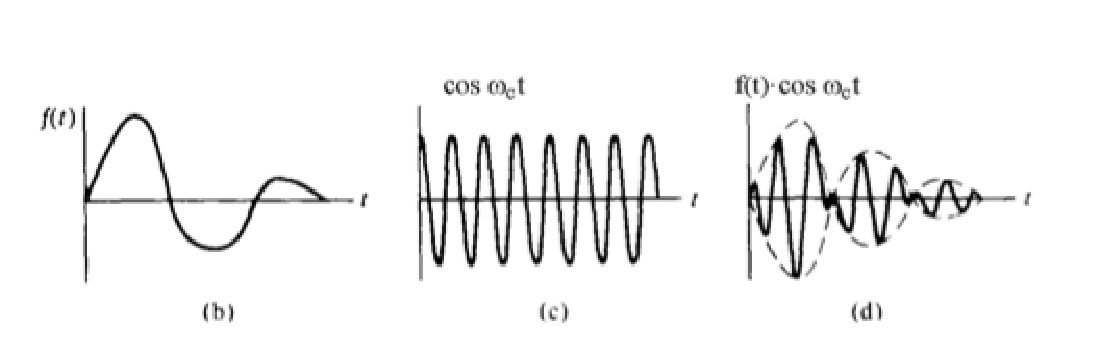
\includegraphics[scale=0.7, trim = 0cm 0cm 0cm 0cm, clip]{./Bilder/AMohneTraeger}
                    \caption{Amplitudenmodulation ohne träger}
                    \label{fig:AMohneTraeger}
                    \cite{AMohnetraeger}
            \end{figure}
    
            Um dieses modulierte Signal am Empfänger wieder zu demodulieren wird es noch ein weiteres mal mit dem
            Trägersignal multipliziert und anschließend Tiefpassgefiltert. Welche Auswirkung das hat zeigt folgendes
            Bild.
            
            \begin{figure}[H]
            \centering
                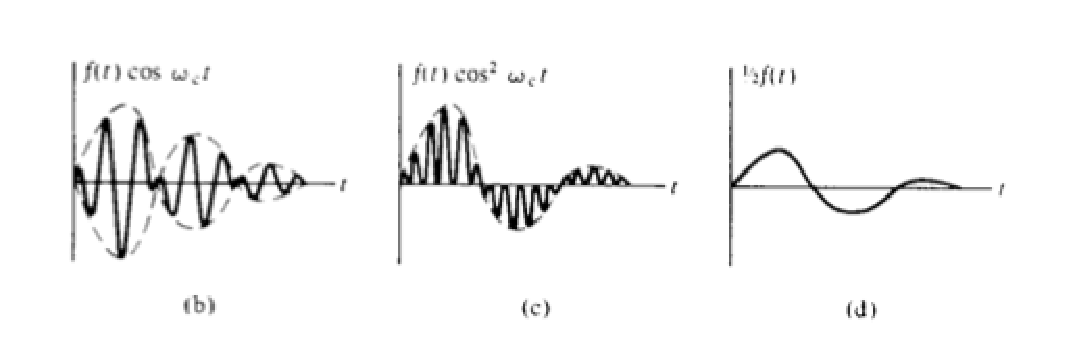
\includegraphics[scale=0.7, trim = 0cm 0cm 0cm 0cm, clip]{./Bilder/AMohnetraegerdemodulation}
                    \caption{Amplitudendemodulation ohne Träger}
                    \cite{AMdemodulation}
            \end{figure}
    
            Die Gesamte Übertragungsstecke der Amplitudenmodulation ohne Träger ist hier zu sehen.
            
            \begin{figure}[H]
            \centering
                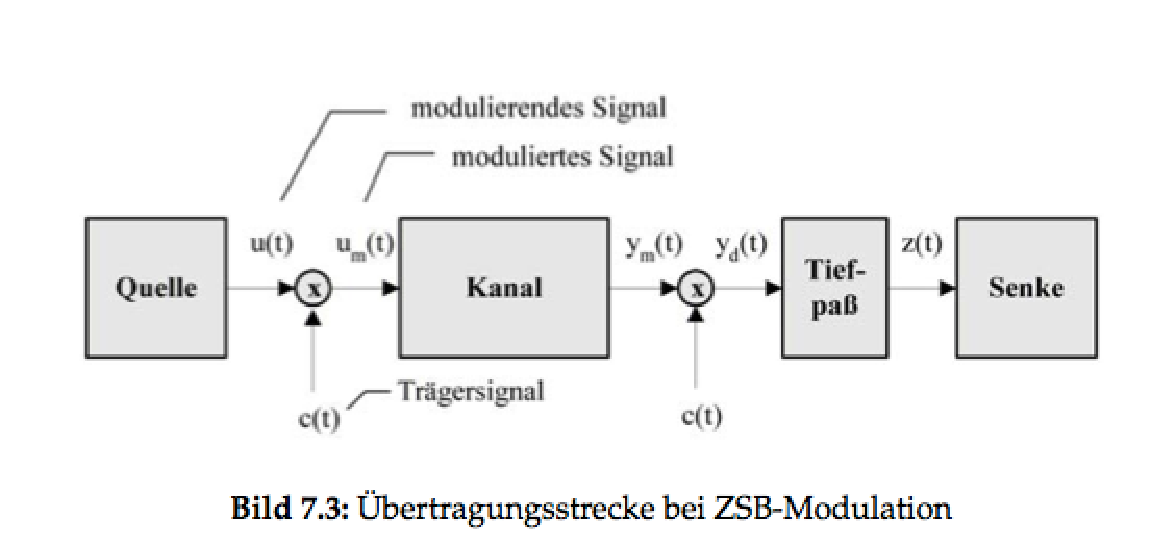
\includegraphics[scale=0.7, trim = 0cm 0cm 0cm 0cm, clip]{./Bilder/uebertragungsstreckeAMohnetraeger}
                    \caption{Übertragungsstrecke AM ohne Träger}
                    \cite{AMohneUeber}
            \end{figure}
             
             Damit diese Modulation jedoch Fehlerfrei funktioniert wird am Empfänger das kohärente Trägersignal
             benötigt. Das Bedeutet, dass das Trägersignal in exakt der selben Phase und Frequenz am Empfänger vorhanden
             sein muss. Ist das nicht der Fall kommt es zur Verfälschung des Nutzsignals bei der Demodulation.\\
             Da das jedoch schwer zu realisieren ist wurde die zweite art der Amplitudenmodulation entwickelt:
             Amplitudenmodulation mit Träger.
             
            
		\end{quote}
		
		\subsubsection{Amplitudenmodulation mit Träger}
		\begin{quote}
			Bei der Amplitudenmodulation mit Träger wird das Nutzsignal $u(t)$ bevor es mit dem Trägersignal $c(t)$
			multipliziert wird mit einem Offset versehen.
			
			\begin{figure}[H]
            \centering
                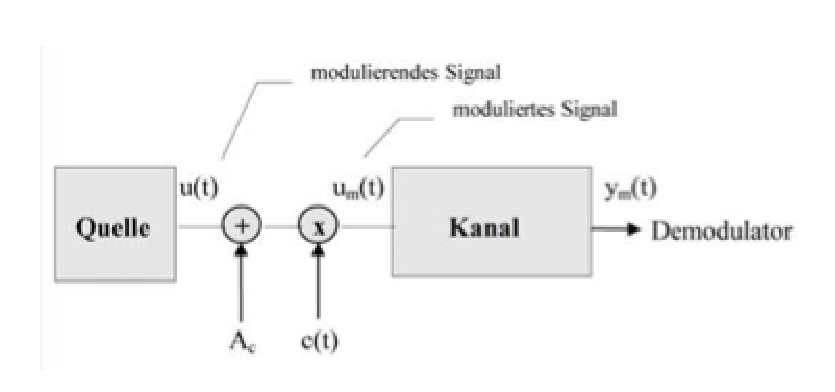
\includegraphics[scale=0.7, trim = 0cm 0cm 0cm 0cm, clip]{./Bilder/AMmitTraeger}
                    \caption{Amplituden Modulation mit Träger}
                    \cite{AMmitUeber}
            \end{figure}
            
            Das bedeutet für die Amplitude des modulierten Signals:
            
            \begin{equation*}
                \begin{split}
                    A_c [u(t)] = A + k \cdot u(t)
                \end{split}
            \end{equation*}
    
		      
		\end{quote}
        
        
    \end{quote}
    
    \subsection{Vorbereitungsaufgabe}
    \begin{quote}
        Als Vorbereitung für die Messungen zum Thema Amplitudenmodulation haben wir mit Hilfe von Matlab verschiedene
        Signalformen simuliert und anschließend Amplituden moduliert.\\
        Dazu haben wir als Nutzsignal jeweils ein Rechtecksignal, ein Dreiecksignal sowie ein Cosinussignal mit
        einer Amplitude (von Nulldurchgang zum Spitzenwert) von $1V$ und einer Frequenz von $100 Hz$. Zusätzlich haben
        wir noch ein Trägersignal mit der selben Amplitude aber mit einer Trägerfrequenz von $2000 Hz$ erstellt.\\
        Anschließend haben wir die drei Nutzsignale Amplitudenmoduliert indem wir sie jeweils mit dem Tägersignal
        multipliziert haben.\\
        Zur Analyse haben abschließende diese modulierten Signale sowie ihre Amplituden- und Phasengänge platten
        lassen.\\
        In der Auswertung werden wir diese Ergebnisse anschließend mit den gemessenen Ergebnissen vergleichen.
    \end{quote}
    
    \subsection{Durchführung}
    \begin{quote}
    	\subsubsection{Signalerzeugung und Modulation}
    	\begin{quote}
    	Als Basisbandsignal generierten wir ein mittelwertfreier Sinus,
    	der eine Frequenz von $100 Hz$ und eine Amplitude von $1 V$ besaß. Dazu wurde noch
    	ein Offset von einem Volt addiert, welches wir mit dem Adder-Modul und der
    	Quelle Variable DCV verwirklicht haben. Somit hatte unser Basisbandsignal
    	keinen Nulldurchgang mehr. Mit den Verstärkerknöpfen g und G wurde die
    	Summe vom Sinus und Offset korrekt eingestellt und am Oszilloskop
    	korrigiert.\\
    	Nachdem unser Nutzsignal erstellt wurde, führten wir die Modulation anhand
    	einer Multiplikation mit dem Multiplier-Modul durch. Als Trägersignal
    	verwendeten wir dabei den $2kHz$-Sinus des Master-Signal-Moduls.\\
    	Nach der Untersuchung des Sinus-Basisbandsignals, wurde die Modulation auf
    	gleiche Weise noch mit dem Rechteck- und dem Dreiecksignal durchgeführt.
    	Die Ergebnisse aus dem Praktikum und der Vergleich mit den Ergebnissen aus
    	der Vorbereitungsaufgabe ist in der Auswertung zu finden.
    	\end{quote}
    	
    	\vspace{1em}
    	
    	\subsubsection{Synchrone Demodulation}
    	\begin{quote}
    	Nach der Amplitudenmodulation wurden die modulierten Signale auch
    	synchron demoduliert. Dies ermöglichten wir mithilfe des zweiten
    	Multiplier-Moduls und indem wir das Trägersignal erneut auf das modulierte
    	Signal multiplizierten. In einem Plot kann man sehen, dass das
    	Empfangssignal die doppelte Amplitude besitzt wie das Sendesignal. Diese
    	Abweichung korrigierten wir anhand eines Vorfaktors von $0.5$ in unserem
    	MATLAB-Skript.
    	
    	Ist das alles richtig so? Ich meine Michael Tok hatte gesagt, dass wir die
    	Halbierung nicht auf dem Steckbrett machen müssen sondern einfach nur in
    	MATLAB ne $\frac{1}{2}$ davor klatschen\ldots \\
    	Die auftretenden Abweichungen erklären wir am Besten auch in der
    	Auswertung.    	
		\end{quote}    
    
    \end{quote}
    
    \subsection{Auswertung}
    \begin{quote}
        
        Hier kann man die Ergebnisse der Amplitudenmodulation sehen. Alle
        Nutzsignale hatten eine Frequenz von $100 Hz$, eine Amplitude von $1 V$
        und einen Offset von ebenfalls $1 V$. Das Trägersignal war ein $2
        kHz$-Sinus.
        
        In die minipages kommen immer die Vorbereitungsergebnisse und die
        Paktikumsergebnisse rein, damit sie miteinander verglichen werden
        können.
        
        
        \begin{center}
            \begin{tabular}{ll}

            \hspace{-14em}
                \begin{minipage}{0.6\textwidth}

                    \begin{figure}[H]
                        \label{fig:}
                        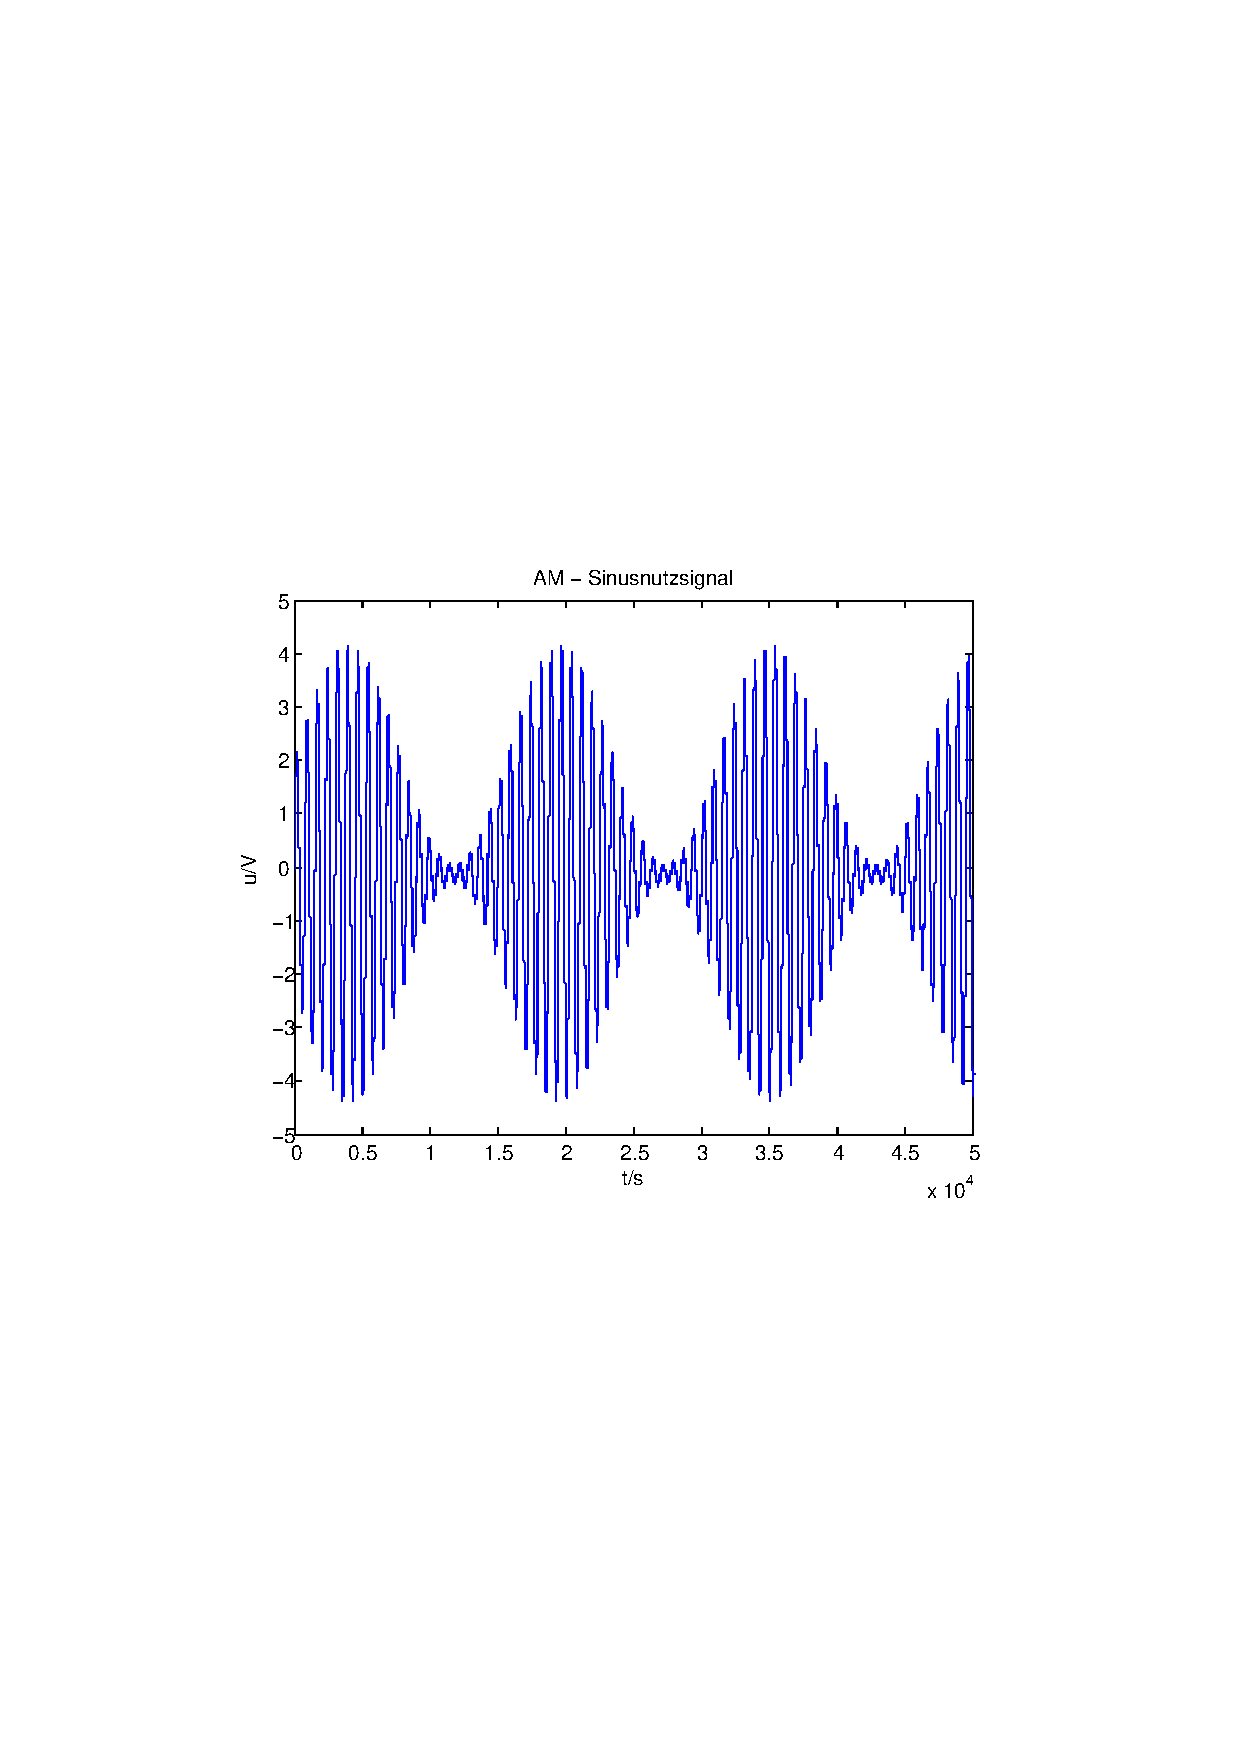
\includegraphics[scale=0.5, trim = 2cm 6.5cm 1.5cm
                        8.5cm, clip]{./Bilder/am-sinus} %FIXME [width=640px,
                        % height=474px]
                        \caption{amplitudenmoduliertes Sinussignal}
                    \end{figure}

                \end{minipage}
                \begin{minipage}{0.6\textwidth}

                     \begin{figure}[H]
                        \label{fig:}
                        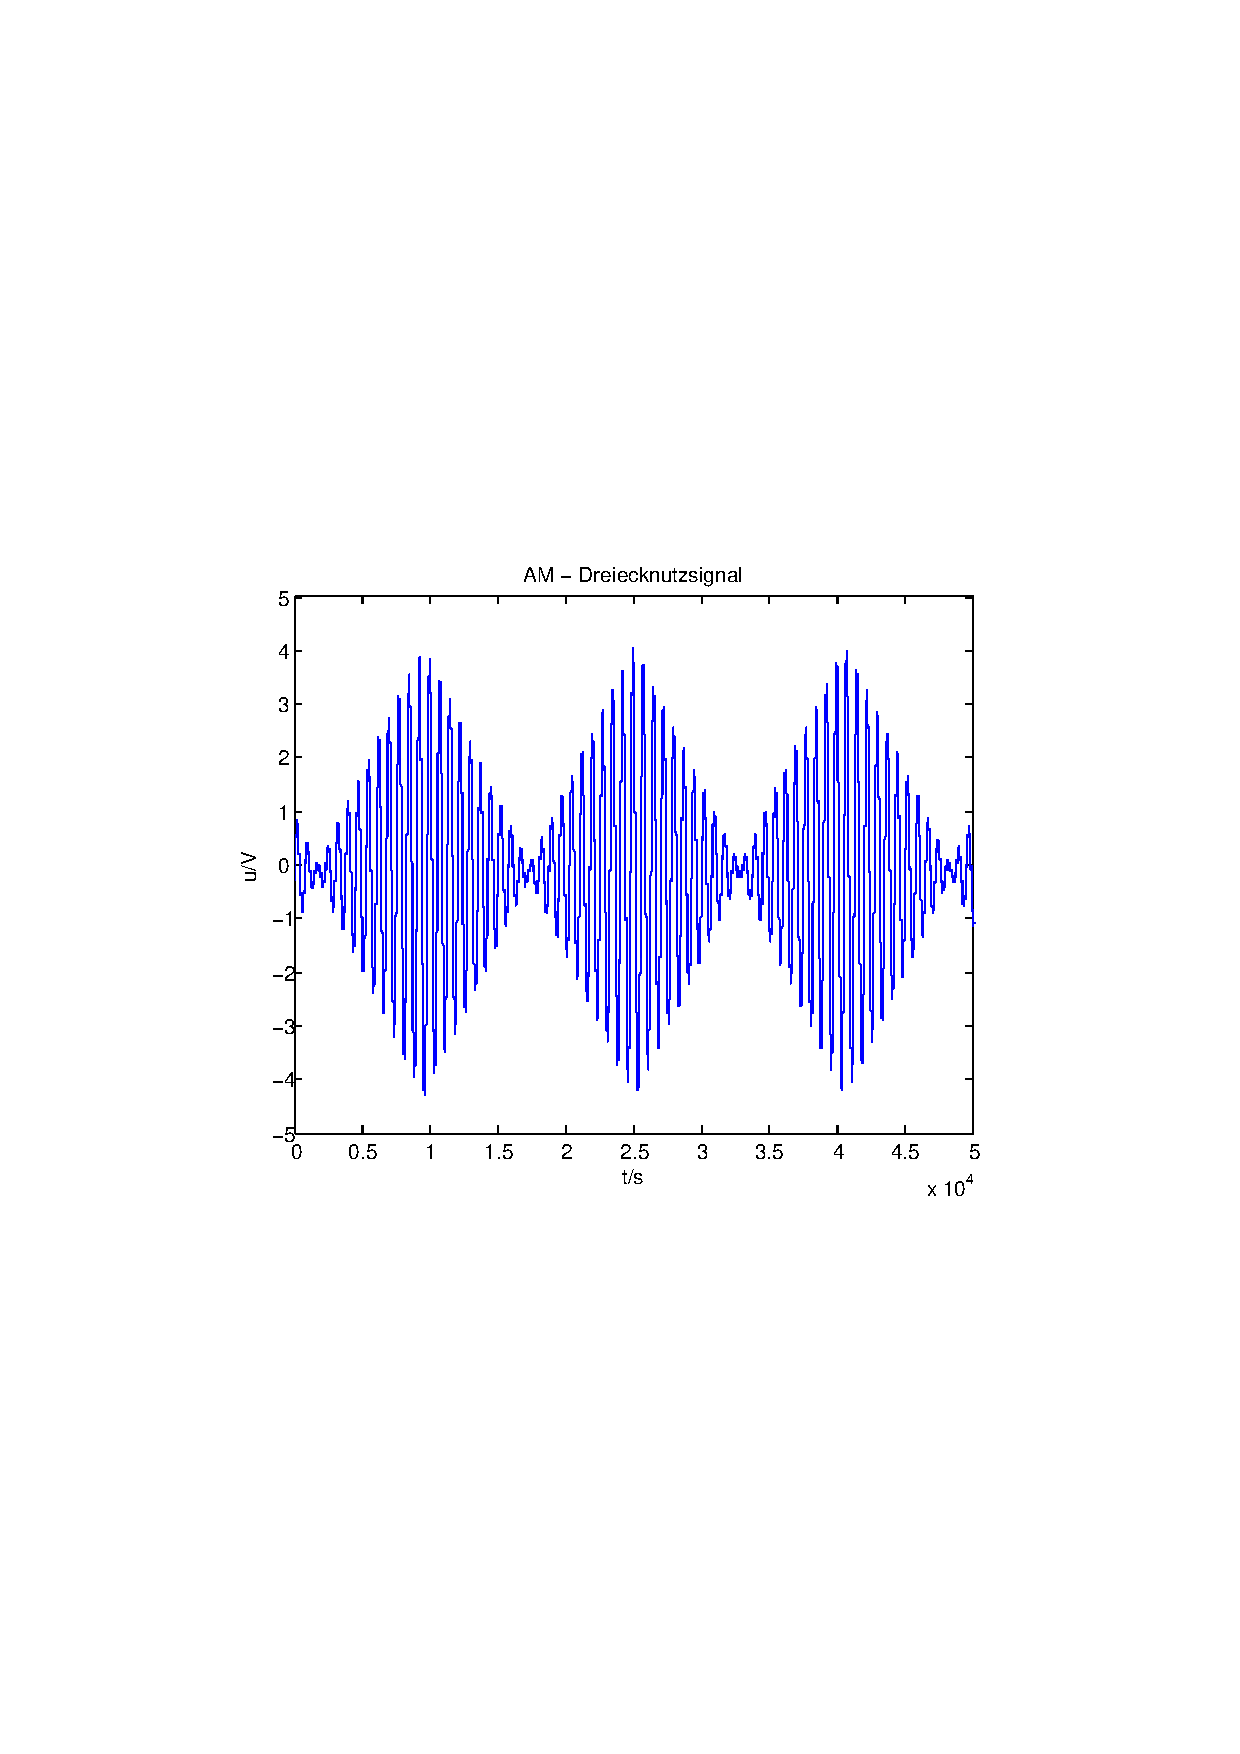
\includegraphics[scale=0.5, trim = 2cm 6.5cm 1.5cm
                        8.5cm, clip]{./Bilder/am-dreieck} %FIXME
                        % [width=640px, height=474px]
                        \caption{amplitudenmoduliertes Dreiecksignal}
                    \end{figure}
               \vspace{-1.5em}

                \end{minipage}

            \end{tabular}
            \end{center}
            
             \begin{figure}[H] \centering
                    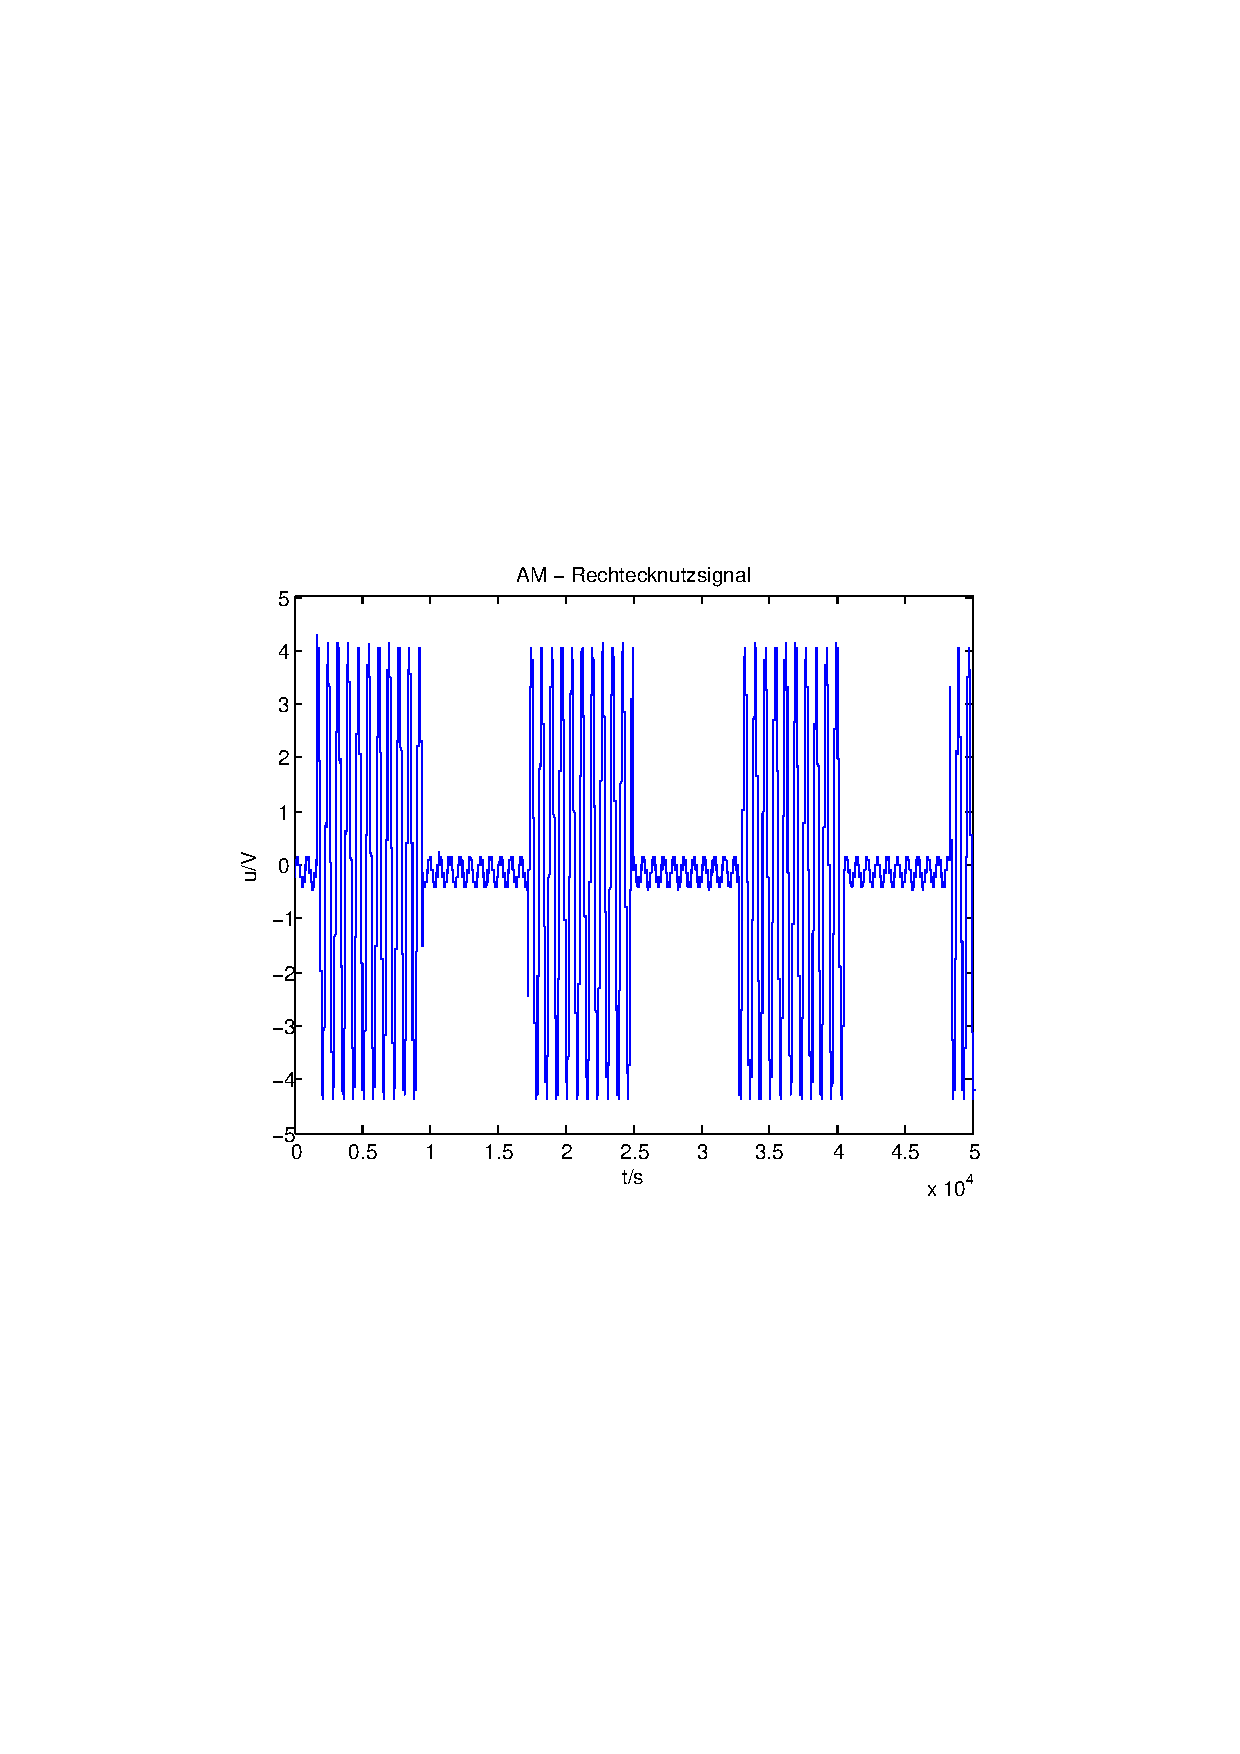
\includegraphics[scale=0.5, trim = 2cm 6.5cm 1.5cm 8.5cm,
                    clip]{./Bilder/am-rechteck}
                        \caption{amplitudenmoduliertes Rechtecksignal}
                \end{figure}
        
    \end{quote}
\end{quote}

%--------------------------------------------------------------------
%--------------------------------------------------------------------            



\section{Frequenzmodulation}
\begin{quote}
    \subsection{Theorie}
    \begin{quote}
        
    \end{quote}
    
    \subsection{Vorbereitungsaufgabe}
    \begin{quote}
     
    \end{quote}
    
    \subsection{Durchführung}
    \begin{quote}
        \subsubsection{Signalerzeugung}
        \begin{quote}
        Als Nutzsignal für die Frequenzmodulation wird ein $3 kHz$-Sinus mit
        einer $1 V$-Amplitude verwendet. Die einfache Modulation verwirklichten
        wir anhand des VCO-Moduls. Dabei wurde der Schalter in der Mitte auf
        die Position LOW gesetzt (das Trägersignal kann damit eine
        Nutzsignalfrequenz zwischen $1 kHz$ und $17 kHz$ annehmbar modulieren),
        der FREQ-Controller auf die mittlere Position gestellt und GAIN auf
        $\approx \frac{2}{3}$ des Maximalwerts gedreht.\\
        Als nächstes wurde das Spektrum des FM-Signals untersucht und die
        Trägerfrequenz $f_c$ sowie die Proportionalitätskonstante $K_{FM}$
        bestimmt. Für die Proportionalitätskonstante gilf folgende Formel:
        
        \begin{equation*}
    	\begin{split}
    		K_{FM} &= \frac{2 \pi \Delta f_{max}}{A_u}\\
			\Delta f_{max} \approx \frac{1}{2} (\frac{1}{T_{min}} - \frac{1}{T_{max}})    		
    	\end{split}
    	\end{equation*}
    	
   		$T_{min}$ und $T_{max}$ bezeichnen dabei die zeitlich kürzeste und längste
   		Periodendauer des Sinussignals.\\
   		Für einen späteren Vergleich wird auch das Spektrum des FM-Signals
   		untersucht, bei der die Nutzfrequenz $f_u = 1 kHz$ und die Nutzamplitude
   		$A_u = 1 V$ beträgt.\\
   		Zusätzlich wurden noch die Nutzsignale mit den Amplituden $0.5 V\, 1 V$ und
   		$2 V$ mit den Frequenzen $50 Hz\, 100 Hz$ und $200 Hz$ frequenzmoduliert
   		und die Spektren des Ausgangs von dem VCO-Modul miteinander verglichen. 
        \end{quote}
        
        \subsubsection{FM-Demodulation}
        \begin{quote}
        Für die folgende FM-Demodulation wurde zunächst die Einstellungen des
        VCO-Moduls verändert. Der Schalter wurde auf HIGH gelegt (nun kann das
        Trägersignal höhere Nutzfrequenzen als $17 kHz$ modulieren), sowie der
        Trägerfrequenz-Drehknopf auf die Hälfte und der GAIN-Drehknopf auf $70
        \%$ eingestellt. Das neu FM-modulierte Sinussignal, mit ursprünglich
        $100 Hz$-Frequenz und $1 V$-Amplitude, wurde dann auf den Eingang des
        Comparator-Moduls gelegt und mit einer Referenzspannung von $0 V$
        verglichen.\\
        
        Die FM-Demodulation erfolgt in diesem Praktikum durch eine
        FM-PFM-Umwandlung (PFM = Pulsfrequenzmodulation). Dabei wandelt der
        Comparator das analoge Signal in ein Standard-Digitalsignal um. Dieses
        besteht aus einer polaren Rechteckfolge, welche dadurch entsteht, dass
        der Comparator jedesmal, wenn das Analogsignal (in diesem Fall der
        von uns verwendete Sinus) das Referenzsignal übersteigt, einen positiven
        Ausgangssignalpegel ausgibt. Wird das Analogsignal kleiner als die
        Referenzspannung wird der Ausgangssignalpegel negativ. Dieses digitale
        Signal wird in den Twin Pulse Generator (TPG) geführt, der aus jeder
        steigenden Flanke ein Rechteckimpuls verwirklicht. Dafür werden die
        Regler DELAY und WIDTH auf ihr Minimum gedreht. Die Pulse des
        entstandenen Rechtecksignals werden abschließend wieder zu einem kontinuierlichen 
        Signalpegel umgewandelt, indem sie durch einen Tiefpass
        (TP) geführt werden.\\
        
        In der Auswertung vergleichen wir zusätzlich die das Sinusquellsignal
        mit dem Comparator-Ausgang, das Sinusquellsignal mit dem Twin Pulse
        Generator-Ausgang und den Comparator-Ausgang mit dem Twin Pulse
        Generator-Ausgang.
         
        \end{quote}
        
    \end{quote}
    
    \subsection{Auswertung}
    \begin{quote}
        
    \end{quote}	
\end{quote}

%--------------------------------------------------------------------
%--------------------------------------------------------------------    

\section{Zusammenfassung}
\begin{quote}
	
\end{quote}

%--------------------------------------------------------------------
%--------------------------------------------------------------------    


\begin{thebibliography}{999}
\bibitem {AMohnetraeger} Prof. Dr.-Ing. Sikora, Thomas; Prof. Dr.-Ing. Noll, Peter: Einführung in die
Nachrichtenübertragung, S.207
\bibitem {AMdemodulation} Prof. Dr.-Ing. Sikora, Thomas; Prof. Dr.-Ing. Noll, Peter: Einführung in die
Nachrichtenübertragung, S.209
\bibitem {AMohneUeber} Prof. Dr.-Ing. Sikora, Thomas; Prof. Dr.-Ing. Noll, Peter: Einführung in die
Nachrichtenübertragung, S.206
\bibitem {AMmitUeber} Prof. Dr.-Ing. Sikora, Thomas; Prof. Dr.-Ing. Noll, Peter: Einführung in die
Nachrichtenübertragung, S.206

%Name, Vorname.; evtl. Name2, Vorname2.: Titel des Dokumentes
%oder Buches, Zeitschrift/Verlag/URL (Auflage, Erscheinungsort, -jahr), ggf. Seitenzahlen
% \bibitem {PasevalscheTheorem} \url{https://de.wikipedia.org/wiki/Parsevalsches_Theorem}, Zugriff
% 23.05.2012
\end{thebibliography}

\end{document}
